\documentclass{beamer}

% ======== BASIC THEME SETUP ========
\usetheme{Madrid}
\useinnertheme{default}
\usecolortheme{default}
\usepackage{tikz}
\usepackage{comment}
\usepackage{graphicx}
\usepackage{booktabs}
\usepackage{array}
\usepackage{listings}
\usepackage{xcolor}
\usepackage{fontawesome5}

\usetikzlibrary{positioning, shapes, arrows.meta}

% ======== CUSTOM COLORS ========
\definecolor{deepNavy}{RGB}{10,15,35}
\definecolor{accentBlue}{RGB}{80,150,255}
\definecolor{softWhite}{RGB}{230,230,230}
\definecolor{mtaRed}{RGB}{238,53,46}
\definecolor{mtaGreen}{RGB}{0,147,60}
\definecolor{mtaOrange}{RGB}{255,99,25}
\definecolor{mtaYellow}{RGB}{252,204,10}
\definecolor{codeGray}{RGB}{25,30,50}

% ======== COLOR SETTINGS ========
\setbeamercolor{background canvas}{bg=deepNavy}
\setbeamercolor{normal text}{fg=softWhite}
\setbeamercolor{frametitle}{fg=white, bg=accentBlue}
\setbeamercolor{title}{fg=accentBlue}
\setbeamercolor{structure}{fg=accentBlue}
\setbeamercolor{itemize item}{fg=accentBlue}
\setbeamercolor{itemize subitem}{fg=mtaRed}
\setbeamercolor{block title}{bg=accentBlue, fg=white}
\setbeamercolor{block body}{bg=codeGray, fg=softWhite}
\setbeamercolor{alerted text}{fg=mtaYellow}

% ======== FRAME TITLE ========
\setbeamertemplate{frametitle}{
	\nointerlineskip
	\begin{beamercolorbox}[wd=\paperwidth,ht=0.65cm,dp=0.3cm,
		leftskip=0.8cm,rightskip=0.8cm,
		colsep*=0pt]{frametitle}
		\usebeamerfont{frametitle}%
		{\color{white}\textbf{\insertframetitle}}
	\end{beamercolorbox}
}

\setbeamercolor{frametitle}{bg=accentBlue, fg=white}
\setbeamerfont{frametitle}{size=\large, series=\bfseries}

% ======== CODE LISTING STYLE ========
\lstdefinestyle{pysmall}{
	backgroundcolor=\color{codeGray},
	commentstyle=\color{accentBlue}\itshape,
	keywordstyle=\color{mtaYellow}\bfseries,
	stringstyle=\color{mtaGreen},
	basicstyle=\ttfamily\scriptsize\color{softWhite},
	breaklines=true,
	frame=none,
	language=Python,
	showstringspaces=false
}

\lstdefinestyle{sqlsmall}{
	backgroundcolor=\color{codeGray},
	commentstyle=\color{accentBlue}\itshape,
	keywordstyle=\color{mtaYellow}\bfseries,
	stringstyle=\color{mtaGreen},
	basicstyle=\ttfamily\scriptsize\color{softWhite},
	breaklines=true,
	frame=none,
	language=SQL,
	showstringspaces=false
}


\graphicspath{{C:/Users/Jujop/Documents/GitHub/mta-transit-pulse/report/figures}}

% Override Madrid's ball-style enumerate items
\setbeamertemplate{enumerate item}{\textcolor{accentBlue}{\textbf{\insertenumlabel.}}}
\setbeamertemplate{enumerate subitem}{\textcolor{mtaRed}{\textbf{\insertenumlabel.}}}
\setbeamertemplate{itemize item}{\textcolor{accentBlue}{\textbf{--}}}
\setbeamertemplate{itemize subitem}{\textcolor{mtaRed}{\small\textbf{--}}}

% ======== CLEANUP ========
\setbeamertemplate{navigation symbols}{}

% ======== FOOTER WITH SLIDE COUNTER ========
\setbeamertemplate{footline}{
	\leavevmode
	\hbox{
		\begin{beamercolorbox}[wd=\paperwidth,ht=2ex,dp=1ex,
			leftskip=1em,rightskip=1em]{footlinecolor}
			\hfill
			\usebeamerfont{footline}%
			\textcolor{accentBlue}{\insertframenumber{} / \inserttotalframenumber}
		\end{beamercolorbox}
	}
}

% ======== TITLE INFO ========
\title{\textbf{MTA Transit Pulse}}
\subtitle{A Data Management Pipeline for NYC Subway Ridership Analysis}
\author{Juan Perez}
\institute{Data Management Course \\ Stony Brook University}
\date{\today}

% ======== BEGIN DOCUMENT ========
\begin{document}
	
	% ------------------------------------------------------------------
	% SLIDE 1 — Title
	% ------------------------------------------------------------------
	\begin{frame}[plain]
		\centering
		\vspace{1.5cm}
		
		{\Large\textcolor{accentBlue}{\textbf{MTA Transit Pulse}}}\\
		\vspace{0.4cm}
		{\small\textcolor{softWhite}{A Data Management Pipeline for NYC Subway Ridership Analysis}}\\
		\vspace{0.8cm}
		\textcolor{accentBlue}{\rule{0.6\textwidth}{0.4pt}}\\
		\vspace{0.6cm}
		{\small\textcolor{softWhite}{Juan Perez}}\\
		\vspace{0.1cm}
		{\scriptsize\textcolor{softWhite}{Data Management Course · Stony Brook University}}\\
		\vspace{0.1cm}
		{\scriptsize\textcolor{softWhite}{\today}}
	\end{frame}
	% ==================================================================
	\section{The Idea}
	% ==================================================================
	
	% ------------------------------------------------------------------
	% SLIDE 3 — The Idea
	% ------------------------------------------------------------------
	\begin{frame}{The Idea}
		\centering
		\Large{\textbf{What if I built a real data pipeline?}}\\
		\vspace{0.5cm}
		\normalsize
		Collect publicly available data published by the Metropolitan
		Transportation Authority (MTA), store it in a relational database,
		and visualize it interactively.\\
		\vspace{0.8cm}
		\pause
		\begin{columns}[c]
			\begin{column}{0.3\textwidth}
				\centering
				\textcolor{accentBlue}{\Large\textbf{120M+}}\\
				\small rows of data
			\end{column}
			\begin{column}{0.3\textwidth}
				\centering
				\textcolor{mtaRed}{\Large\textbf{428}}\\
				\small unique stations
			\end{column}
			\begin{column}{0.3\textwidth}
				\centering
				\textcolor{mtaGreen}{\Large\textbf{5 years}}\\
				\small 2020 -- 2024
			\end{column}
		\end{columns}
	\end{frame}
	
	% ------------------------------------------------------------------
	% SLIDE 4 — Pipeline overview (your existing timeline, cleaned up)
	% ------------------------------------------------------------------
\begin{frame}{The Objective}
	Build an end-to-end data pipeline that pulls real MTA subway data, cleans and stores it in a local database, analyzes patterns and trends, and visualizes the results in a dashboard.
	
	\vspace{0.8cm}
	\centering
	\scalebox{0.8}{
		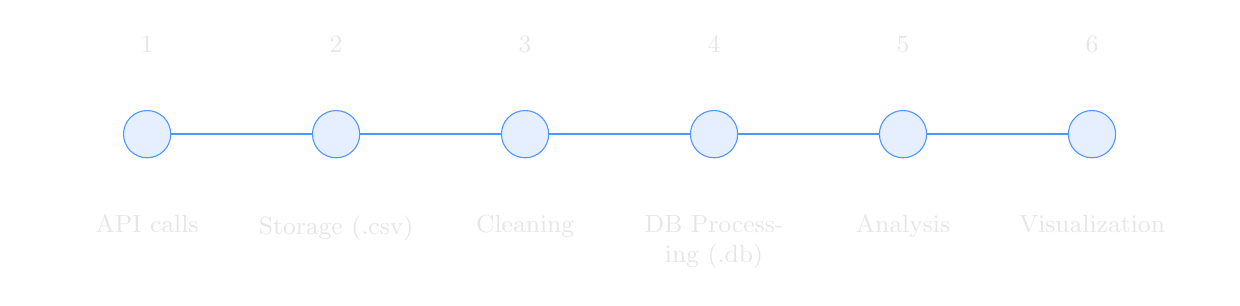
\begin{tikzpicture}[
			timeline/.style={
				thick,
				accentBlue
			},
			event/.style={
				circle,
				draw=accentBlue,
				fill=accentBlue!15,
				minimum size=6mm,
				inner sep=2pt
			},
			textstyle/.style={
				text width=2.8cm,
				align=center,
				font=\small,
				softWhite
			}
			]
			
			% Timeline line
			\draw[timeline] (0,0) -- (12,0);
			
			% Events (nodes)
			\node[event] (A) at (0,0) {};
			\node[event] (B) at (2.4,0) {};
			\node[event] (C) at (4.8,0) {};
			\node[event] (D) at (7.2,0) {};
			\node[event] (E) at (9.6,0) {};
			\node[event] (F) at (12,0) {};
			
			% Labels below timeline
			\node[textstyle, below=0.6cm of A] {API calls};
			\node[textstyle, below=0.6cm of B] {Storage (.csv)};
			\node[textstyle, below=0.6cm of C] {Cleaning};
			\node[textstyle, below=0.6cm of D] {DB Processing (.db)};
			\node[textstyle, below=0.6cm of E] {Analysis};
			\node[textstyle, below=0.6cm of F] {Visualization};
			
			% Labels above timeline
			\node[textstyle, above=0.6cm of A] {1};
			\node[textstyle, above=0.6cm of B] {2};
			\node[textstyle, above=0.6cm of C] {3};
			\node[textstyle, above=0.6cm of D] {4};
			\node[textstyle, above=0.6cm of E] {5};
			\node[textstyle, above=0.6cm of F] {6};
			
		\end{tikzpicture}
	}
	
	\vspace{0.8cm}
	\centering
	\textit{\small Cronological setup}
	
\end{frame}

	
	% ==================================================================
	\section{The Dataset}
	% ==================================================================
	
	% ------------------------------------------------------------------
	% SLIDE 5 — Dataset overview (your existing slide, refined)
	% ------------------------------------------------------------------
	\begin{frame}{The Dataset}
		\centering
		\textbf{MTA Subway Hourly Ridership: 2020--2024}\\
		\vspace{0.3cm}
		{\small\textcolor{accentBlue}{data.ny.gov · dataset ID: wujg-7c2s}}
		
		\vspace{0.4cm}
		\resizebox{\textwidth}{!}{
			\begin{tabular}{@{}>{\bfseries\color{accentBlue}}l
					>{\color{softWhite}}p{0.85\textwidth}@{}}
				\toprule
				Column & Description \\
				\midrule
				transit\_timestamp   & Hour in which the tap/swipe occurred (rounded down) \\
				transit\_mode        & Subway, Staten Island Railway, or Roosevelt Island Tram \\
				station\_complex\_id & Unique identifier for each station complex \\
				borough              & One of the five NYC boroughs \\
				payment\_method      & OMNY or MetroCard \\
				fare\_class\_category& Consolidated fare type (11 categories) \\
				ridership            & Total riders entering at this hour via this fare type \\
				latitude / longitude & Station complex coordinates \\
				\bottomrule
			\end{tabular}
		}
	\end{frame}
	
	% ------------------------------------------------------------------
	% SLIDE 6 — Why this dataset?
	% ------------------------------------------------------------------
	\begin{frame}{Why This Dataset?}
		\begin{columns}[T]
			\begin{column}{0.48\textwidth}
				\textcolor{accentBlue}{\textbf{Strengths}}
				\begin{itemize}
					\item Real, production-grade data
					\item Pre-cleaned by the MTA (deduplicated, validated)
					\item Rich schema: time, location, fare type
					\item Spans COVID collapse \& recovery (2020--2024)
					\item Free, public APIt
				\end{itemize}
			\end{column}
			\begin{column}{0.48\textwidth}
				\textcolor{mtaRed}{\textbf{Challenges}}
				\begin{itemize}
					\item 120M rows (memory management required)
					\item API returns all values as \textbf{strings}
					\item Undocumented \texttt{georeference} column caused schema mismatch on first load
					\item Default API limit: 1,000 rows, token required
				\end{itemize}
			\end{column}
		\end{columns}
	\end{frame}
	
	% ==================================================================
	\section{Data Collection}
	% ==================================================================
	
	% ------------------------------------------------------------------
	% SLIDE 7 — collect.py
	% ------------------------------------------------------------------
	\begin{frame}[fragile]{Stage 1 — Data Collection (\texttt{collect.py})}
		\textbf{Approach:} SODA2 REST API with paginated requests\\
		\vspace{0.3cm}
		\begin{block}{Query parameters sent on every request}
			\begin{lstlisting}[style=pysmall]
params = {
	"$limit" : 500_000,   # rows per page
	"$offset": offset,    # advances each page
	"$where" : "transit_timestamp >= '2020-01-01T00:00:00'",
	"$order" : "transit_timestamp ASC"
}

headers = {"X-App-Token": TOKEN}  # loaded from .env
			\end{lstlisting}
		\end{block}
		\vspace{0.2cm}
		\begin{itemize}
			\item \textbf{240 API requests} to collect all 5 years
			\item Each page saved as \texttt{raw\_page\_NNN.csv}
			\item \textbf{Resume capability}: skips pages already on disk
			\item 1s to 10s delay between requests to avoid throttling
		\end{itemize}
	\end{frame}
	
	% ==================================================================
	\section{Cleaning \& Storage}
	% ==================================================================
	
	% ------------------------------------------------------------------
	% SLIDE 8 — clean.py
	% ------------------------------------------------------------------
	\begin{frame}[fragile]{Stage 2 — Cleaning (\texttt{clean.py})}
		\textbf{Design principle:} raw data is not modified — clean data
		is a separate product written to \texttt{data/clean/}\\
		\vspace{0.3cm}
		\textcolor{accentBlue}{\textbf{Memory strategy:}} process one page (500K rows) at a time
		\begin{itemize}
			\item Peak RAM: $\approx$50MB regardless of total dataset size
			\item Output: one \texttt{clean\_YEAR.csv} per year ($\approx$5GB each)
		\end{itemize}
		\vspace{0.3cm}
		\textcolor{accentBlue}{\textbf{Steps applied per page:}}
		\begin{enumerate}
			\item Cast \texttt{ridership} \& \texttt{transfers} to numeric
			\item Drop \texttt{georeference} (redundant with lat/lon columns)
			\item Remove nulls in critical columns
			\item Remove ridership $< 0$ or $> 100{,}000$
			\item Strip whitespace from string columns
			\item Derive \texttt{date}, \texttt{hour}, \texttt{day\_of\_week}
			\item Deduplicate
		\end{enumerate}
	\end{frame}
	
	% ------------------------------------------------------------------
	% SLIDE 9 — db.py and load.py
	% ------------------------------------------------------------------
	\begin{frame}[fragile]{Stage 3 — Database (\texttt{db.py} + \texttt{load.py})}
		\begin{columns}[T]
			\begin{column}{0.48\textwidth}
				\textcolor{accentBlue}{\textbf{Schema (SQLite)}}
				\begin{block}{}
					\begin{lstlisting}[style=sqlsmall]
CREATE TABLE IF NOT EXISTS
	ridership (
	id INTEGER PRIMARY KEY,
	transit_timestamp TEXT,
	station_complex   TEXT,
	borough           TEXT,
	payment_method    TEXT,
	fareclass_category TEXT,
	ridership   INTEGER,
	date        TEXT,
	hour        INTEGER,
	day_of_week TEXT
	);
					\end{lstlisting}
				\end{block}
			\end{column}
			\begin{column}{0.48\textwidth}
				\textcolor{accentBlue}{\textbf{Loading strategy}}
				\begin{itemize}
					\item Chunks of 500K rows via \texttt{pd.read\_csv(chunksize)}
					\item Loading process done per year
					\item WAL mode enabled for bulk write performance
					\item 3 indexes created: \texttt{date}, \texttt{station}, \texttt{hour}
				\end{itemize}
				\vspace{0.3cm}
				\textcolor{mtaGreen}{\textbf{Final result:}}\\
				\textbf{120,855,567 rows} · 0 nulls in critical columns
			\end{column}
		\end{columns}
	\end{frame}
	
	% ------------------------------------------------------------------
	% SLIDE 10 — Data quality verification
	% ------------------------------------------------------------------
	\begin{frame}[fragile]{Data Quality Verification}
		\centering
		\textit{First queries run after loading to check on integrity}\\
		\vspace{0.15cm}
		\begin{block}{Row count by year}
			\begin{lstlisting}[style=sqlsmall]
SELECT strftime('%Y', transit_timestamp) AS year,
COUNT(*) AS rows
FROM ridership
GROUP BY year ORDER BY year;
			\end{lstlisting}
		\end{block}
		\vspace{0.15cm}
		\resizebox{0.35\textwidth}{!}{
			\begin{tabular}{@{}
					>{\color{accentBlue}\bfseries}c
					>{\color{softWhite}}r@{}}
				\toprule
				Year & Rows \\
				\midrule
				2020 & 20,339,851 \\
				2021 & 23,281,980 \\
				2022 & 24,635,810 \\
				2023 & 25,585,413 \\
				2024 & 27,012,513 \\
				\midrule
				\textbf{Total} & \textbf{120,855,567} \\
				\bottomrule
			\end{tabular}
		}\\
	\end{frame}
	
	% ==================================================================
	\section{Analysis}
	% ==================================================================
	
	% ------------------------------------------------------------------
	% SLIDE 11 — Analysis questions
	% ------------------------------------------------------------------
	\begin{frame}{Analysis — Six Questions}
		\centering
		\textit{All queries executed in .ipynb via \texttt{pd.read\_sql\_query()}}\\
		\vspace{0.5cm}
		\begin{enumerate}
			\item[\textcolor{accentBlue}{\textbf{Q1}}]
			Which 10 station complexes have the highest total ridership?
			\item[\textcolor{mtaRed}{\textbf{Q2}}]
			How does ridership vary by \textbf{hour of day}?
			\item[\textcolor{mtaGreen}{\textbf{Q3}}]
			Which \textbf{day of the week} is busiest?
			\item[\textcolor{mtaOrange}{\textbf{Q4}}]
			How does ridership compare across \textbf{boroughs}?
			\item[\textcolor{mtaYellow}{\textbf{Q5}}]
			How has \textbf{OMNY} adoption grown vs MetroCard over time?
			\item[\textcolor{accentBlue}{\textbf{Q6}}]
			What does the \textbf{COVID recovery} look like year over year?
		\end{enumerate}
	\end{frame}
	
	% ------------------------------------------------------------------
	% SLIDE 12 — Q1 + Q4 results (stations + boroughs)
	% ------------------------------------------------------------------
	\begin{frame}{Q1 \& Q4 — Stations and Boroughs}
		\begin{columns}[T]
			\begin{column}{0.5\textwidth}
				\textcolor{accentBlue}{\textbf{Top 5 stations by total ridership}}
				\vspace{0.2cm}
				\resizebox{\textwidth}{!}{
					\begin{tabular}{@{}>{\color{softWhite}}l
							>{\color{mtaYellow}\bfseries}r@{}}
						\toprule
						Station & Total Riders \\
						\midrule
						Times Sq--42 St & 1.68B \\
						Grand Central--42 St & 1.15B \\
						34 St--Herald Sq & 974M \\
						14 St--Union Sq & 866M \\
						Fulton St & 707M \\
						\bottomrule
					\end{tabular}
				}
				\vspace{0.3cm}
				
				\small Penn Station appears \textbf{twice} under different line groupings (A/C/E and 1/2/3)
			\end{column}
			\begin{column}{0.5\textwidth}
				\textcolor{accentBlue}{\textbf{Borough comparison}}\\
				\vspace{0.2cm}
				% Insert your borough chart here:
				
\includegraphics[width=\textwidth]{top_ridership_borough.png}
			\end{column}
		\end{columns}
	\end{frame}
	
	% ------------------------------------------------------------------
	% SLIDE 13 — Q2 + Q3 results (hourly + daily patterns)
	% ------------------------------------------------------------------
	\begin{frame}{Q2 \& Q3 — Temporal Patterns}
		\begin{columns}[T]
			\begin{column}{0.5\textwidth}
				\textcolor{accentBlue}{\textbf{Ridership by hour of day}}\\
				\vspace{0.2cm}
				
\includegraphics[width=\textwidth]{total_ridership_per_hour.png}
				\small Classic double-peak: \textbf{08:00} morning rush,
				\textbf{17:00--18:00} evening rush
			\end{column}
			\begin{column}{0.5\textwidth}
				\textcolor{accentBlue}{\textbf{Ridership by day of week}}\\
				\vspace{0.2cm}
				
\includegraphics[width=\textwidth]{total_ridership_per_day.png}
				\small \textbf{Friday} is the busiest day —
				weekends show a clear drop vs weekdays
			\end{column}
		\end{columns}
	\end{frame}
	
	% ------------------------------------------------------------------
	% SLIDE 14 — Q5 OMNY vs MetroCard
	% ------------------------------------------------------------------
	\begin{frame}{Q5 — OMNY vs MetroCard Adoption}
		\centering
		
\includegraphics[width=0.85\textwidth]{omny_vs_metrocard.png}
		\vspace{0.2cm}
		
		\small
		OMNY launched in 2019. By 2024 it accounts for a \textbf{majority} of
		all subway rides — MetroCard adoption is in clear decline as the MTA
		phases out the legacy system.
	\end{frame}
	
	% ------------------------------------------------------------------
	% SLIDE 15 — Q6 COVID recovery
	% ------------------------------------------------------------------
	\begin{frame}{Q6 — COVID-19 Ridership Recovery}
		\centering
		
\includegraphics[width=0.85\textwidth]{covid_recovery.png}
		\vspace{0.2cm}
		
		\small
		Ridership collapsed in March 2020, reaching its lowest point during lockdowns. The dataset captures the full recovery arc —
		\textbf{2024 ridership is the highest in this dataset} at 27M rows,
		surpassing pre-pandemic baselines on many lines.
	\end{frame}
	
	% ==================================================================
	\section{Visualization}
	% ==================================================================
	
	% ------------------------------------------------------------------
	% SLIDE 16 — Streamlit dashboard
	% ------------------------------------------------------------------
	\begin{frame}{Streamlit Dashboard}
		\textbf{Three interactive pages — all querying live from SQLite}\\
		\vspace{0.4cm}
		\begin{columns}[T]
			\begin{column}{0.32\textwidth}
				\centering
				\textcolor{accentBlue}{\textbf{Station Explorer}}\\
				\vspace{0.2cm}
				\small
				Pick any of 428 stations.\\
				See hourly \& daily\\
				ridership profile.\\
				Filter by year.
			\end{column}
			\begin{column}{0.32\textwidth}
				\centering
				\textcolor{mtaRed}{\textbf{System Trends}}\\
				\vspace{0.2cm}
				\small
				Network-wide patterns.\\
				Peak hours, busiest days,\\
				borough comparison,\\
				top 10 stations.
			\end{column}
			\begin{column}{0.32\textwidth}
				\centering
				\textcolor{mtaGreen}{\textbf{Recovery Timeline}}\\
				\vspace{0.2cm}
				\small
				Year-over-year recovery\\
				from COVID-19.\\
				OMNY adoption curve.\\
				Fare class breakdown.
			\end{column}
		\end{columns}
		\vspace{0.5cm}
		\begin{block}{Key design decisions}
			\begin{itemize}
				\item \texttt{@st.cache\_data} on all queries — avoids re-querying
				120M rows on every user interaction
				\item Parameterized SQL queries — no string interpolation with
				user input
			\end{itemize}
		\end{block}
	\end{frame}
	
	% ==================================================================
	\section{Challenges}
	% ==================================================================
	
	% ------------------------------------------------------------------
	% SLIDE 17 — Engineering challenges
	% ------------------------------------------------------------------
	\begin{frame}{Engineering Challenges I}
		\begin{enumerate}
			\item \textcolor{accentBlue}{\textbf{Memory management}}\\
			\small 120M rows cannot fit in RAM simultaneously.
			Solution: page-by-page cleaning — never more than 50MB in memory
			at once regardless of total dataset size.\\[0.3cm]
			
			\item \textcolor{mtaRed}{\textbf{Undocumented column}}\\
			\small The API returned a \texttt{georeference} column absent from
			the official data dictionary. This caused a schema mismatch on
			first load. Fix: drop it during cleaning with
			\texttt{errors=``ignore''}.\\[0.3cm]
			
			\item \textcolor{mtaGreen}{\textbf{Type coercion}}\\
			\small The SODA2 API returns every value as a string.
			Without explicit \texttt{pd.to\_numeric()} casting,
			numeric comparisons and datetime operations silently fail.\\[0.3cm]
			
		\end{enumerate}
	\end{frame}
	
		\begin{frame}{Engineering Challenges II}
		\begin{enumerate}
			
			
			\item[\textbf{4.}] \textcolor{mtaYellow}{\textbf{Transaction performance}}\\
			\small Initial load tests showed slow inserts.
			Wrapping each year in a single transaction and enabling
			WAL mode reduced load time \textbf{5--10$\times$}.\\[0.3cm]
			
			\item[\textbf{5.}] \textcolor{mtaOrange}{\textbf{API resume capability}}\\
			\small A 240-request collection can crash halfway through.
			Solution: check for existing page files before each request
			and skip if already downloaded.
		\end{enumerate}
	\end{frame}
	
	% ==================================================================
	\section{Conclusions}
	% ==================================================================
	
	% ------------------------------------------------------------------
	% SLIDE 18 — Key findings
	% ------------------------------------------------------------------
	\begin{frame}{Key Findings}
		\vspace{0.2cm}
		\begin{itemize}
			\item \textbf{Times Square--42 St} is the busiest complex in the system
			by a wide margin — \textcolor{mtaYellow}{\textbf{1.68 billion riders}}
			over 5 years
			\vspace{0.2cm}
			\item The subway shows a clear \textbf{double-peak pattern} daily:
			08:00 and 17:00--18:00, with a valley between 02:00--05:00
			\vspace{0.2cm}
			\item \textbf{Manhattan} accounts for the overwhelming majority of
			system-wide ridership, followed by Brooklyn
			\vspace{0.2cm}
			\item \textbf{OMNY} has overtaken MetroCard as the dominant payment
			method by 2024 — a complete payment ecosystem transition
			captured in the data
			\vspace{0.2cm}
			\item Ridership grew \textbf{+32.8\%} from 2020 to 2024, confirming
			near-complete post-COVID recovery visible directly in the numbers
			\vspace{0.2cm}
			\item \textbf{Friday} is consistently the busiest day of the week —
			weekends carry noticeably fewer riders than weekdays
		\end{itemize}
	\end{frame}
	
	% ------------------------------------------------------------------
	% SLIDE 19 — What we built / tech stack
	% ------------------------------------------------------------------
	\begin{frame}{Tools used}
	
			\textcolor{accentBlue}{\textbf{Tech stack}}
			\begin{itemize}
					\item \textbf{Python 3.13} — pipeline scripts
					\item \textbf{pandas} — data cleaning \& transformation
					\item \textbf{SQLite} — 23GB relational database
					\item \textbf{Streamlit} — interactive dashboard
					\item \textbf{matplotlib} — analysis charts
					\item \textbf{python-dotenv} — secure credential handling
					\item \textbf{Git + GitHub} — version control
				\end{itemize}
	\end{frame}
	
	% ------------------------------------------------------------------
	% SLIDE 20 — Future work + closing
	% ------------------------------------------------------------------
	\begin{frame}{Future Work \& Closing}
		\begin{columns}[T]
			\begin{column}{0.55\textwidth}
				\textcolor{accentBlue}{\textbf{If this project were extended:}}
				\begin{itemize}
					\item Real-time GTFS delay feeds to correlate ridership
					drops with service disruptions
					\item NOAA weather enrichment — does rain increase
					ridership on certain lines?
					\item PostgreSQL migration for multi-user access
					\item Automated weekly ingestion via GitHub Actions —
					triggered every Monday when MTA publishes new data
					\item Station-level geospatial map using
					\texttt{latitude} / \texttt{longitude} columns
				\end{itemize}
			\end{column}
			\begin{column}{0.42\textwidth}
				\centering
				\vspace{0.5cm}
				\textcolor{accentBlue}{\rule{\textwidth}{0.4pt}}\\
				\vspace{0.4cm}
				{\Large\textbf{MTA Transit Pulse}}\\
				\vspace{0.3cm}
				{\small\textcolor{softWhite}{
						120,855,567 rows\\
						428 stations · 5 boroughs\\
						2020 -- 2024\\
				}}
				\vspace{0.3cm}
				{\scriptsize\textcolor{accentBlue}{
						github.com/jujopo/mta-transit-pulse
				}}\\
				\vspace{0.3cm}
				\textcolor{accentBlue}{\rule{\textwidth}{0.4pt}}\\
				\vspace{0.5cm}
				{\large\textbf{Thank you}}\\
				{\small Questions?}
			\end{column}
		\end{columns}
	\end{frame}
	
\end{document}